\documentclass[iop]{emulateapj}
\let\captionbox\relax
\usepackage{graphicx}
\bibliographystyle{yahapj}

%define general packages
\usepackage{epsfig}
\usepackage{rotating}
\usepackage{amsmath}
\usepackage{footnote}
\usepackage{courier}
\usepackage{color}
\usepackage{subfigure}



\begin{document}
\title{Ultraviolet to Infrared Star Formation Rate Indicators and Galaxy Environment}
\author{Nityasri Mandyam\altaffilmark{1} and Michael R. Blanton\altaffilmark{1}}
\altaffiltext{1}{Center for Cosmology and Particle Physics, Department of Physics, New York University, New York, NY $10003$}
\begin{abstract}
Star-forming galaxies preferentially populate isolated regions, while 
non-star-forming galaxies preferentially exist in groups and clusters. 
We investigate how this relationship depends on the star formation 
rate indicator using full UV to IR photometry for a local sample 
of galaxies (redshift $z \sim 0.05$) with ultraviolet and optical 
photometry from the NASA Sloan Atlas and infrared photometry 
from WISE. We measure the Specific Star Formation Rates (SSFR) 
in two independent ways: (a) using MAGPHYS, a complete UV to IR 
SED fitting method that models dust absorption and emission; (b) 
using purely the UV light to quantify star formation rates and 
accounting for dust attenuation from the ratio of fluxes in FUV 
and NUV bands. We estimate environments using projected 
aperture densities and distances to the $n^{th}$ nearest 
neighbor. We find that SSFR as measured including the infrared 
emission is more closely related to the galaxy environments 
than the UV indicator. Specifically, galaxies with high SSFR
but with significant dust-obscuration  cluster like 
non-dust-obscured galaxies with high SSFR. These findings are 
consistent with MAGPHYS faithfully accounting for the effect of
dust on the UV and IR emission, and with the clustering of star
forming galaxies being independent of their dust obscuration.
\end{abstract}
\keywords{}
\section{Introduction}

Determining the formation history of galaxies is one of the most important 
tasks in astronomy. The average star formation rates of galaxies 
have reduced with cosmic time (as reviewed by Madau $2014$) and
star-forming galaxies ``transition" to red and quiescent ones (e.g., 
\cite{ilbert_mass_2013, muzzin_evolution_2013, moustakas_primus:_2013, tomczak_galaxy_2014} among others).
Many mechanisms have been proposed to explain the observed patterns of 
galaxy  evolution but there are many unresolved questions regarding them. 
These mechanisms are known to have a some correlation with the environment, 
due to the fact that galaxy type depends on environment in the present day
(\citealt{hubble36a, dressler80a}, and many others).

Star formation rate estimates are an important tool in the observational
study of this problem (see the review of \citealt{kennicutt12a}). 
Spectroscopic indicators contain signatures of star 
formation in them; however, often a spectrum of the galaxy is not 
readily available and we have to rely on converting photometric fluxes 
to meaningful star formation estimates. In this paper we compare 
two specific ways to estimate star formation rates from photometry.
The first is to fit physical models including stellar population
models and dust to the spectral energy distribution 
(SED) of each galaxy using photometric data in various available band-passes.
The second is to use the far and near UV fluxes to estimate a 
dust-extinction-corrected UV luminosity and thus star formation 
rate. 

The presence of dust is an important complication in this analysis.
Dust absorbs preferentially in the UV/optical region of the galaxy 
spectrum and both extincts and reddens the photometric data. This 
energy is re-emitted in the mid- to far-IR by poly-cyclic aromatic 
hydrocarbon molecules as well as warm and cold grains.
Recent studies (\citet{Burg13}) find that in the nearby universe, 
almost $70\%$ of the FUV luminosity is obscured by dust on an 
average. Although UV estimates of star formation do attempt to 
account for dust attenuation\underline{(Such as \citet{salim_uv_2007} and)}, 
the extensive reliance on UV SFR in the literature 
(\underline{cite Peng et al, Moustakas et al..?}) makes it 
important to understand the extent to which the dust corrections 
for UV SFR estimates work relative to other methods of estimating SFR.

Here, we examine a sample of galaxies whose UV-IR photometry 
is available and estimate the star formation rate in two independent 
ways. First we exploit the fact that we have UV to IR photometry 
and perform SED fitting using MAGPHYS \cite{da_cunha_simple_2008}, which 
accounts for dust by using a simple method of energy balance to 
obtain the specific star formation rates (SSFRs). The other method 
involves using purely UV photometry to estimate both star 
formation rate and dust attenuation using the prescription given 
by \citet{salim_uv_2007}. We also estimate the environments of our population.

We ask the following questions of this sample. How do these 
different star formation estimators disagree with each other? 
How does each estimate correlate with environment? Does
one  trace environment more closely? 
Under the assumption that the environment primarily 
correlates with the SSFR rather than dust obscuration's effect
on the observables, studying this correlation will yield 
insights into the relative accuracy of the methods.

\begin{figure*}
    \centering
	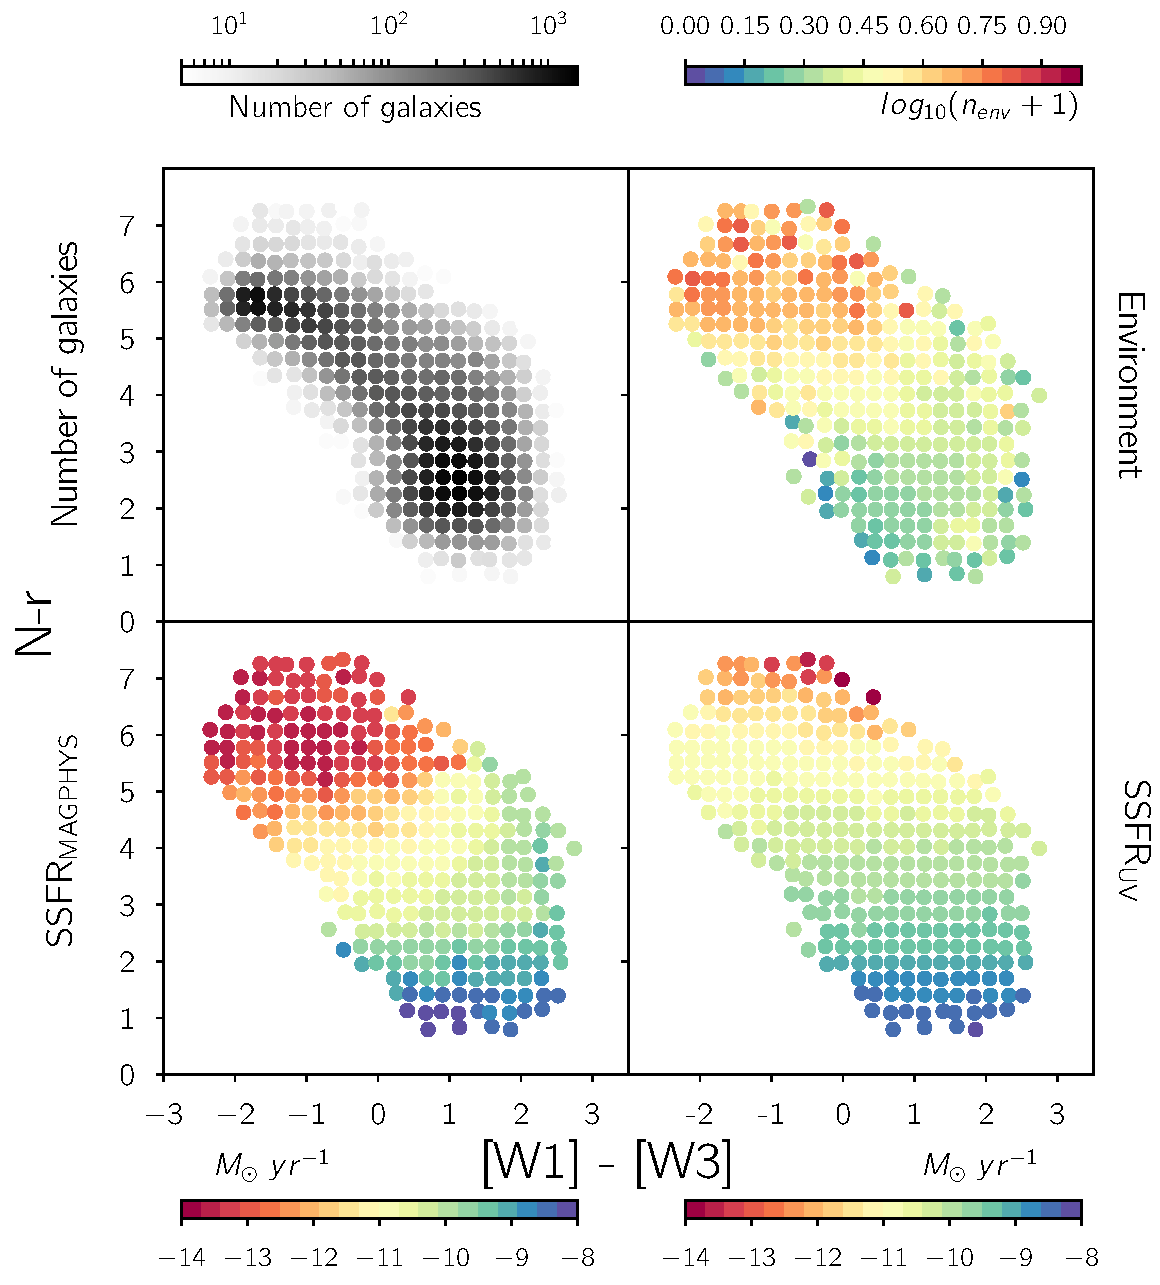
\includegraphics[width = 16 cm, height = 16 cm]{1_panel_plot.pdf}
	\caption{The SSFR measurements and environment shown the color-color 
    space. Each point in the plot is shown at the mean colors in each of 
    the bins we use. The grey value or color of the points in each
    panel show the mean value in each bin for the quantity described 
    by the corresponding  color bar.
    \emph{Top left:} Logarithmic number density in each of the 
    bins; all bins with less than $5$ galaxies were discarded in this 
    and the other panels. \emph{Top right:} Environment; in each bin, 
    the average number of nearest neighbors is calculated in a 
    projected cylinder ($r_{t} = 0.5 Mpc$ and $v_{los} = \pm 1000 km/s$). 
    \emph{Bottom left:} the Specific Star Formation Rates obtained from 
    MAGPHYS. \emph{Bottom right:} UV Specific Star Formation Rates 
    estimated by using the method described in \citet{salim_uv_2007}.} 
\end{figure*}

\section{Data}

\subsection{Constructing a local sample spanning Ultraviolet to Infrared Imaging}

The sample on which we perform our measurements is based on the NASA-Sloan 
Atlas, a nearby galaxy sample which includes optical and ultraviolet 
imaging from SDSS and GALEX. We use the currently public version 
of the NSA (http://nsatlas.org) whose redshift range extends up 
to $z = 0.055$ and includes SDSS (Data Release $9$) and GALEX 
imaging for galaxies. The total number of objects in the NSA 
catalog is $\sim 150,000$. We define two samples from the NSA, one that we use to define environment(Environment Determining Population or EDP, hereafter) and one for which we determine star 
formation rates (Star Formation Rate Population or SFRP hereafter). We note that the SFRP is a subsample of the EDP. To get our EDP, we impose a volume-limited cut on this sample by retaining only galaxies with $-24.5 <M_{r}< -18.5$ which leaves us with $95,638$ galaxies. 


The star formation rate determinations we use here
require both UV data and IR data. About 80\% of our 
galaxies have UV data from GALEX analyzed in the NSA.
To obtain infrared imaging for the data we have 
matched the objects from the NSA with the WISE (Wide-Field Infrared 
Survey Explorer) data \textbf{which catalog specifically? ALLWISE DR $2013$?}
with $K$-corrected WISE magnitudes. 
Now about $20\%$ of the objects in the NSA do not have GALEX Photometry, which is crucial for us to determine our SFR's, especially the UVSFR's. Apart from that, less than $1\%$ of the objects do not have reasonable optical/WISE fluxes. We removed all such objects with missing/faulty photometry in addition to correcting for edges in sample \textbf{(refer section Edge Effects)}. Since we intend to study the evolution of these galaxies through the optical-IR phase space, we imposed a cut in optical ($7.5> N-r >=0 $) and infrared ($3.0> [W1]- [W3] >= -3.0$) colors (top left corner of Fig. $1$). Our SFRP ultimately consists of $61,046$ objects with absolute magnitudes in the UV ($F$ and $N$ bands), optical ($U$,$g$,$r$,$i$ and $z$ bands) and infrared ($W1$,$W2$, $W3$ and $W4$ bands). \textbf{How was K-correction done for WISE?} \\

 
The environment tracing sample needs to be volume-limited; that is,
to have an expected mean density independent of redshift. To
achieve this, we restrict in absolute magnitude to
$-18.5 > M_{r}  > -24.5$. This yields a
population of $95,638$ galaxies. 
zero/negative fluxes,  to obtain $75476$
galaxies upon which the star formation rate measurements were 
then performed. \textbf{is this last sentence still right?}\\

\section{Estimating the Specific Star Formation Rates}

We compare two approaches to calculating specific star formation rates (SSFRs). 
The first uses UV, optical, and IR data. The second uses only the UV data.

\subsection{SED Fitting - MAGPHYS}

We develop here a method to quickly estimate SSFRs based on UV-optical
and infrared colors. We begin by sorting galaxies into bins of the 
$N-r$ - $[W1]-[W3]$ color space ($25\times25$; \textbf{what is size of
bins in magnitudes}). Within each bin, we normalize the fluxes of 
each galaxy relative to a constant flux in the $r$-band, and then 
take the mean normalized flux in each band over all galaxies in the 
bin. This procedure yields a ``template" SED for each bin in the 
color-color space.\\

We then use Multi-wavelength Analysis of Galaxy Physical Properties 
\cite[MAGPHYS]{daC08} to infer the SSFR for each template SED. MAGPHYS
is a simple, largely empirical but physically motivated model to 
interpret the mid- and far-infrared spectral energy distributions
of galaxies consistently with the emission at ultraviolet, optical,
and near-infrared wavelengths. For every input galaxy with a set 
of observed fluxes in different bands, MAGPHYS generates an 
optical and infrared library at that redshift and then samples 
all template spectra whose fluxes obey a simple principle of 
energy balance: that the amount of energy absorbed by dust 
in the UV/Optical matches \underline{within some tolerance?} 
the amount of infrared emission that is accounted for purely 
by dust. Once the templates have been sub-sampled thus, 
MAGPHYS uses chi-squared fitting to see which combination 
best reproduces the observed fluxes along with the likelihood 
for the distributions.\\

\begin{figure}
	\centering
		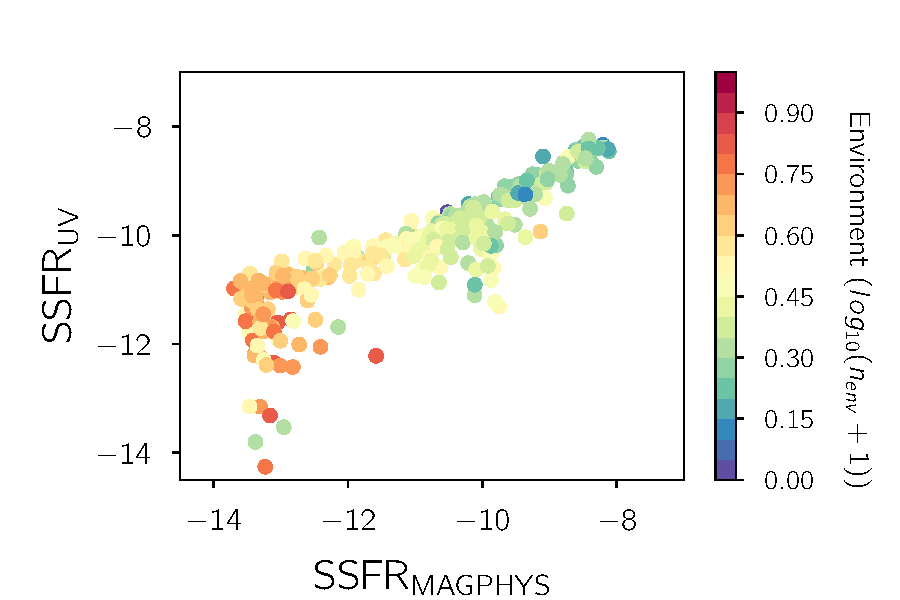
\includegraphics[width = 9 cm, height = 6.0 cm]{2_env_plot.pdf}
	\caption{The two star formation rate estimates (from Fig.$1$) plotted against each other as a function of the environment; We notice two distinct set of outliers that seem to have lower UV SSFR's but similar environments to the galaxy bins with the same MAGPHYS SSFR's.} 
\end{figure}

The results for the SSFRs thus obtained for each template are shown 
in the lower left panel of Figure $1$ along with the number 
distribution of the galaxies across the chosen bins. Note that 
bins with $< 5$ galaxies 
were omitted as those regions of the color-color space are 
obviously under-sampled. \\

The resulting distribution of the MAGPHYS-based SSFRs across the 
color-color space looks as we would expect it to for the most part.
In UV-optical colors, blue galaxies have high SSFRs, and 
red galaxies have low SSFRs. 
However, there is also a dependence of SSFR on IR color; most notably,
in the UV-optical green valley, the redder galaxies in the IR have
higher SSFRs. These galaxies are likely to be dust-extincted in the 
UV, with the reemission by dust reddening the IR colors.

In what follows, we will use the UV-optical and IR colors of individual
galaxies, and the dependence of the SSFR on these colors shown in 
the lower left panel of Figure 1, to assign an SSFR to each individual
galaxy.

\subsection{UV Star Formation Rates}

We also explore a simple method of determining star formation rates
developed by  \citet{salim_uv_2007} that depends only on the UV fluxes of 
each galaxy. It assigns a star formation rate that is proportional 
to the UV luminosity (specifically the FUV band if we are looking at 
GALEX). Dust attenuation is also accounted for in this method by 
looking at the ratio of luminosities in the FUV and NUV bands.\\

\begin{figure*}
	\centering
		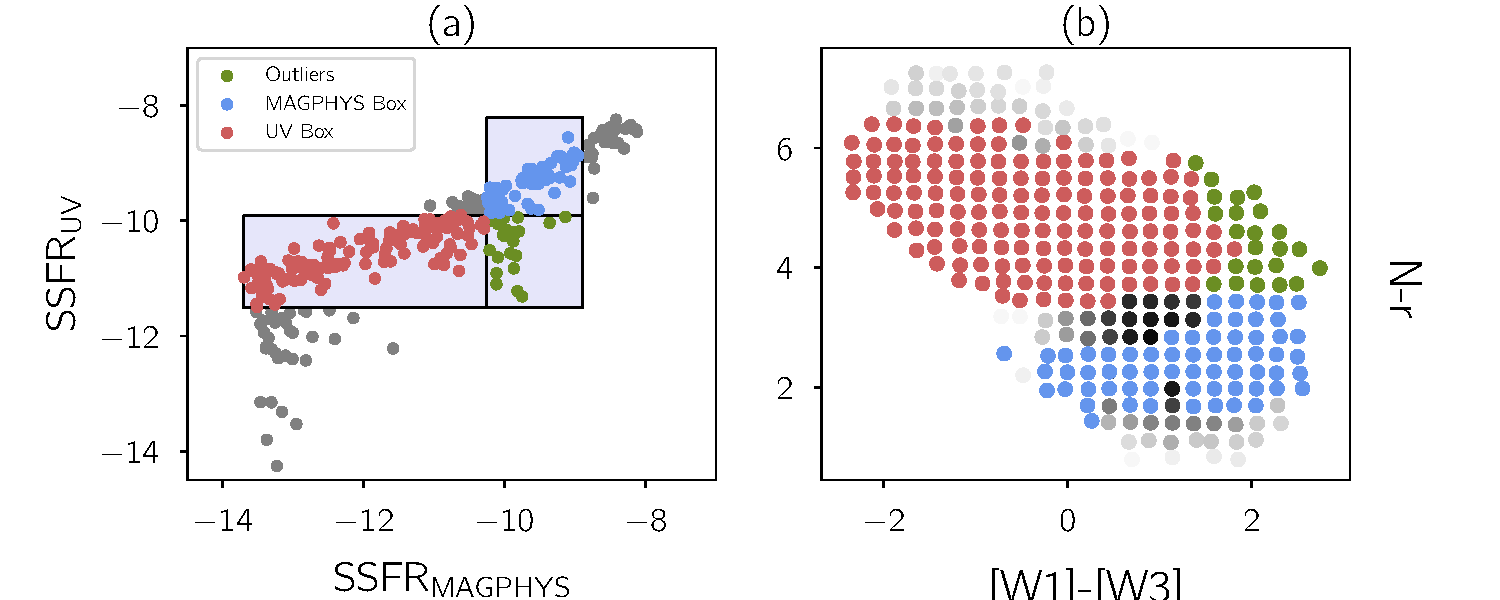
\includegraphics[width = 16 cm, height = 6.4 cm]{3_outliers.pdf}
	\caption{The outliers shown as a function of the Star Formation Rates as well as Optical and IR colors} 
\end{figure*}

According to this prescription \citep{salim_uv_2007}, the star formation 
rate is given by:
$$ SFR = 1.08 \times 10^{-28}{L^{0}}_{\rm FUV} $$
Where ${L^{0}}_{FUV}$ is the rest-frame FUV luminosity. This 
method accounts for dust attenuation of the FUV light as well by 
estimating an attenuation factor $A_{\nu}$ as 
follows.

If $N-r \geq 4.0$, i.e. for the red sequence galaxies,\\
$$ A_{\nu} = 
\begin{cases} 3.32 (F-N) + 0.22, & \text{if} (F-N) < 0.95\\
3.37, & \text{if} (F-N) \geq 0.95 
\end{cases}$$

And if $N-r < 4.0$ , i.e. for the blue sequence galaxies,\\
$$A_{\nu} = 
\begin{cases} 2.99(F-N) + 0.27, & \text{if}(F-N) < 0.90\\
2.96, & \text{if} (F-N) \geq 0.90 
\end{cases}$$\\

This method effectively uses the UV slope to estimate the 
dust attenuation.

The lower right panel of Fig. $1$ shows the mean UV SSFR as 
a function of color. Compared to the lower left panel, the UV 
SSFR's have a nearly monotonic relationship with UV-optical color 
whereas, as discussed above, the  MAGPHYS SSFRs do not. 
Assuming the MAGPHYS SSFRs are closer to correct, the UV-optical green 
valley contains a population of galaxies that are not truly transitioning 
but instead are reddened by the presence of dust. Furthermore, the nominally
dust-corrected UV star formation rates do not successfully identify
these galaxies. \textbf{it seems like a good idea to quantify the 
fraction of galaxies like this; say within $2.5 < N-r < 4.5$, what fraction
have $W1-W3 > 1.5$, or something like that. might be good to answer 
that question in 3 bins of absolute magnitude too}

\section{Environments}

We identified above a population of galaxies isolated in color space,
which appeared to have dust-extincted star formation, such that the UV SSFR estimate
was much less than the MAGPHYS SSFR.
In order to confirm whether MAGPHYS is capturing an inherent  property of
in this population of galaxies, we examine an independent physical property, 
namely the environments of our sample.\\

\subsection{Measures of Environment}

The environment of a galaxy can be defined in many ways, such as 
fixed aperture counts, distance to the $n^{th}$ nearest neighbor, 
Voronoi volumes, etc \cite[]{Coop06}. Here we use counts in a 
projected fixed aperture of radius $0.5$ Mpc as our environment
measure. Around every galaxy we construct a projected cylinder
with a radius (in the transverse direction) of $r_{t} = 0.5$ 
Mpc and a line of sight velocity window of 
$v_{los} = \pm 1000 km/s$. We count the number of 
neighbors ($n_{\rm env}$) in this cylinder(Fig. $1,2$) from the Environment 
Defining Population.

\subsection{Edge Effects}

We must also account for the survey edges. For galaxies at the edge, 
part of the fixed aperture used to estimate the environments might 
lie outside the survey coverage. It is important to identify these
galaxies and either discard them or assign an appropriate weight to 
$n_{\rm env}$ in order to account for the missing area. 

\textbf{I think the following couple of paragraphs could be shortened}

To identify the edges, we use (Swanson et. al.'s \textbf{find citation}) 
\texttt{Mangle}, a suite of free open-source software designed 
to deal with complex angular masks in an efficient and accurate 
manner. First, the NYU-VAGC mask was used to obtain the angular 
mask for the NASA Sloan Atlas by using the \emph{polyid} 
routine from \texttt{Mangle}. Then, the \emph{ransack} 
routine was used to populate the mask with a random sample of 
$N = 10,000,000$ galaxies.

For each galaxy, we compute the angular separation 
$\theta_{i}$ that corresponds to our $0.5 Mpc$ aperture at 
the redshift of that galaxy. We then count the number of 
galaxies $n_{i}$ that lie within this angular separation 
and compare the value obtained to the expected value 
(Hahn et. al.): $$\big \langle n \big \rangle _{i} = 
\frac{N}{A_{\mathrm{EDP}}} \times \pi \theta_{i}^{2} 
\times f_{\mathrm{thresh}} $$

$A_{\mathrm{EDP}}$ is the total area of the mask and 
$f_{\mathrm{thresh}}$ is the fractional threshold for the 
edge effect cut-off. In our case, we chose $f_{\mathrm{thresh}} = 0.8$. 
Wherever $n_{i} < \big \langle n \big \rangle _{i} $, 
we consider the galaxy to be near an edge and discard it 
from our sample. ($\%$ removed from our sample?)

\subsection{Environments in Color-Color Space}

The mean environment, quantified by $(\langle n_{\rm env}\rangle + 1)$
in each bin are shown in the upper right panel of Fig. $1$ as a function 
of optical and infrared colors. As we expect from many previous studies, 
i.e., the star-forming bluer galaxies tend to exist in less dense 
environments on an average and the red-and-dead population tends 
to exist in more dense environments. In the UV-optical green valley region
($3 < N-r < 5$) there is some indication that the environment declines 
with $[W1]-[W3]$ color at fixed UV-optical color. However, the 
mean environments in this plot cannot easily be interpreted, because
the mean stellar mass in each bin is different, so some of the variation
is driven by the dependence of environment on stellar mass.

\section{The Environments of the Outliers}

Fig. 2 shows the relationship between the two SSFR 
measurements as a function of environment
for each bin in color-color space from Fig. 1. The color
indicates the environments. 
There is a set of bins in the range 
$ -10.5 < \mathrm{MAGPHYS} \mathrm{SSFR} < -9.5$ that 
have lower UV SSFRs than the general trend line, and 
have environments similar to the other galaxy bins 
in the same MAGPHYS range. Hereafter we shall refer 
to this population as the ``Outliers", to distinguish 
them from the general trend line in Fig. $2$. 

We proceed to identify these more concretely in 
Fig. $3(a)$. The galaxy bins with the same MAGPHYS 
SSFR's are identified as the ``MAGPHYS Box" and 
the bins with the same UV SSFR's are identified as 
``UV BOX" in Fig. $3(a)$. \\

\begin{figure}
	\centering
		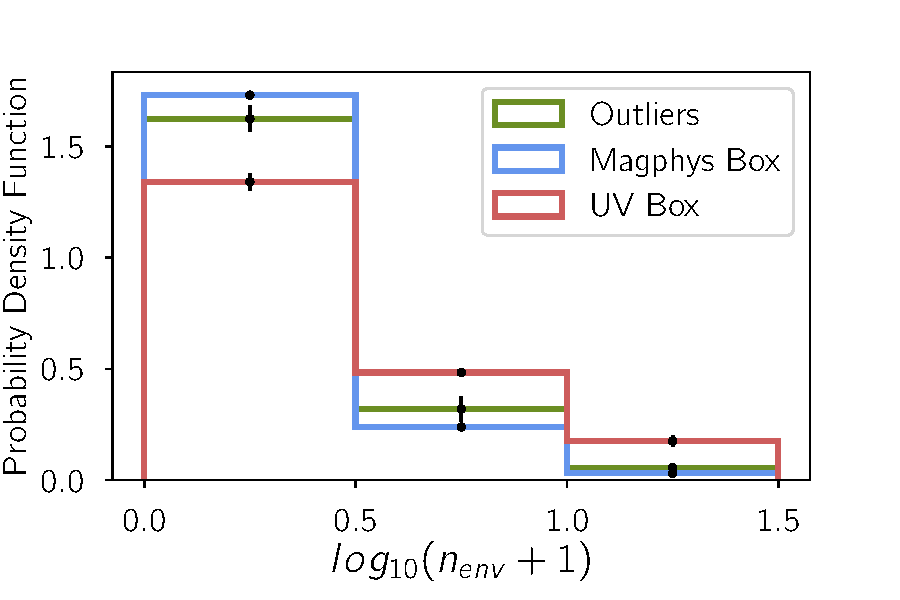
\includegraphics[width = 9 cm, height = 6.0 cm]{4_jk_plot.pdf}
	\caption{Probability density functions of the Environments of the three populations described in Fig. $2$; } 
\end{figure}

When we return to the color-color space (Fig. $3(b)$) and show
where the bins in each box lie,  we see the trends we would expect. 
The Outliers  lie in a similar UV-optical color range as the UV box 
but have higher IR color. The MAGPHYS Box occupies the bluer side 
in the optical color range while spanning almost the entire IR color range. 
The UV Box occupies the redder side in the optical color range while 
having lower IR color values. The Outlier bins are the 
same bins we previously identified as the galaxies in 
the UV-optical ``green valley" that are there due to dust reddening. 

\textbf{the paragraph below deserves a lot more detail and its own section}

To verify this, we unwrap the bins and look at the Probability 
Density Function of the Environments of the galaxies in these three regions in the mass range  $ 9.5 < M_{*} < 10.7$ and the result of that is plotted in Fig. $4$.

\subsection{Jackknife Errors}

To calculate uncertainty in the estimated probability density 
functions of the environments, $P_{i,\mathrm{bin}}$'s : 
$i = 1,2,3$ for each of the populations, we use the standard 
jackknife technique. Jackknife re-sampling gives us an internal 
error estimate that tests how representative a measurement/trend 
is of the data it is estimated with. We divide our entire 
sample into $20$ subsamples with nearly equal co-moving 
volumes and estimate the same probability density 
functions($P^{j}_{i}$'s) for the whole sample while leaving 
out one subsample each time. We can then estimate our uncertainty 
for each bin in the PDF's thus:
$$ \sigma_{i, \mathrm{bin}} = \sqrt{\sum_{j = 1}^{j = 20} (P^{j}_{i} - P_{i,bin})^{2}} $$
The errors estimated in this manner account for Poisson shot
noise and also the sample variance, the extra error associated
with the fact that the density field varies across the survey. 
Although precision studies of large scale structure have found
that latter effect is not perfectly accounted for with standard
jackknife techniques, they are precise enough for our purposes
here. The jackknife errors are shown in Fig. $4$ and confirm our 
hypothesis: that the Outliers are a little different than the 
MAGPHYS Box but still, very different from the UV Box.

\section{Summary and Conclusion}


\begin{itemize}
\item{From Fig $1$, we see that MAGPHYS SSFR identifies a region in the color-color space as dust-obscured star forming galaxies and correlates better with the environments of the galaxies.}
\item{At the higher star formation end, we find that the dust-obscured star-formers as identified by MAGPHYS have environments comparable to the blue star-forming galaxies, confirming that this is indeed a physical effect we're seeing.}
\item{Comparing the environment distribution of the Outliers relative to the galaxies with (a) the same MAGPHYS SSFR's as the Outliers and (b) the same UV SSFR's as the Outliers (Fig. $4$), we find that the Outliers indeed have a similar environment distribution to the galaxies that have the same MAGPHYS SSFR's, i.e., they seem to favor lower environment densities mimicking the behavior of star-formers.}
\end{itemize}


\bibliography{ref}

%\begin{thebibliography}{}
%
%\bibitem[Bruzual, G., \& Charlot, S.(2003)]{Bru03} Bruzual, G., \& Charlot, S. 2003, \mnras, 344, 1000
%\bibitem[Burgarella, D. et al.(2013)]{Burg13} Burgarella, D., Buat, V., \& Gruppioni, C., et al. 2013, \aa, 554, A70
%\bibitem[Calzetti, D., Kinney, A. L., \& Storchi-Bergmann, T. (1994)]{Cal94}Calzetti, D., Kinney, A. L., \& Storchi-Bergmann, T. 1994, \apj, 429, 582
%\bibitem[Chabrier, G. (2003)]{Chab03} Chabrier, G. 2003, \pasp, 115, 763
%\bibitem[Charlot, S. \& Fall, S. M. (2000)]{Char00}Charlot, S., \& Fall, S. M. 2000, \apj, 539, 718
%\bibitem[Cooper M. C. et al.(2006)]{Coop06} Cooper M. C. et al., 2006, \mnras, 370, 198
%\bibitem[da Cunha, E. et al. (2008)]{daC08} da Cunha, E., Charlot, S., \& Elbaz, D. 2008 \mnras, 388, 1595
%\bibitem[Ilbert, O., McCracken, H. J., Le Fe`vre, O., et al. 2013, A&A, 556, A55
%\bibitem[Kennicutt, R. (1983)]{Ken83}Kennicutt, R. 1983, \textcolor{red}{\aj}, 120, 219
%\bibitem[Kennicutt, R. C., Jr. (1998)]{Ken98} Kennicutt, R. C., Jr. 1998, \araa, 36, 189
%\bibitem [Madau P. et. al. (1998)]{Mad98} Madau, P., Pozzetti, L., \& Dickinson, M. 1998, \apj, 498, 106
%\bibitem[Salim, S. et al.(2007)]{Sal07} Salim, S., Rich, R. M., Charlot, S., et al., 2007, \apjs, 173, 267
%\end{thebibliography}

\end{document}